\documentclass[a4paper,12pt]{report}
\usepackage{graphicx}
\usepackage{times}
\usepackage[a4paper,total={6in,8in}]{geometry}
\usepackage{multirow}
\usepackage{caption}
\usepackage{blindtext}

\begin{document}

{\centering \bf \large
	WORKLORD\par
}
\begin{center}
	{\small PROJECT REPORT} \vspace*{10pt}
	\\ Submitted by\\
	\vspace*{15pt}
	{\bf MOHAMMED ALTHAF T\\
\vspace*{8pt}	LKMC18MCA026\\

\vspace*{8pt}ANJUSHA BJ\\
\vspace*{8pt}KMC18MCA002\\
	\vspace*{20pt}
	to}\\
	\vspace*{13pt}
	the APJ Abdul Kalam Technological University in partial fulfillment of
	the requirements for the award of the Degree\\
	\vspace*{10pt} of\\
	\vspace*{10pt} \textit{ Master of Computer Applications
	} 
\vspace*{10pt}
\begin{figure}[bph]
	\centering
	
\includegraphics[width=0.3023\linewidth]{kmct}
	\label{fig:ksblogo}
\end{figure}

	\bf{Department of Management Studies  Computer Applications
	\vspace*{15pt}
	\\KMCT College of Engineering
	\vspace*{10pt}
	\\Kallanthode, NITC P.O, Kozhikode-673601}

\end{center}
	\begin{center}
		\vspace*{15pt}AUGUST 2020
	\end{center}


\pagebreak


{\centering \bf \large
	DECLARATION\par
}

\vspace*{20pt}
{\normalsize I undersigned here by declare that the project report “{\bf WORKLORD}”, submitted for partial fulfillment of the requirements for the award of degree of Master
	of Computer Applications of the APJ Abdul Kalam Technological University, Kerala is a bonafide
	work done by me under supervision of Mr. Ajayakumar K K. This submission represents my ideas in my
	own words and where ideas or words of others have been included, I have adequately and accurately
	cited and referenced the original sources. I also declare that I have adhered to ethics of academic
	honesty and integrity and have not misrepresented or fabricated any data or idea or fact or source
	in my submission. I understand that any violation of the above will be a cause for disciplinary action
	by the institute and/or the University and can also evoke penal action from the sources which have
	thus not been properly cited or from whom proper permission has not been obtained. This report
	has not been previously formed the basis for the award of any degree. } \\


\hspace*{15pt} \hfill ANJUSHA BJ \\

\hspace*{0pt} \hfill Signature..................... \\
\vspace*{10pt} Place: Kallanthode \\
\vspace*{10pt} Date: 27/8/2020 \\ 
\hspace*{0pt} \hfill MOHAMMED ALTHAF T \\

\hspace*{0pt} \hfill Signature.....................
	
	
\pagebreak

\begin{center}
	
\textbf{
\vspace*{8pt}
DEPARTMENT OF MANAGEMENT STUDIES \& COMPUTER
\vspace*{8pt}
APPLICATIONS\\
KMCT COLLEGE OF ENGINEERING\\
\vspace*{8pt}
Kallanthode, NITC P.O, Kozhikode-673601
}

\begin{figure}[bph]
	\centering
	
\includegraphics[width=0.3023\linewidth]{kmct}
	\label{fig:ksblogo}
\end{figure}
\end{center}

{\centering \bf \large
	CERTIFICATE\par
}
\vspace*{10pt}
This is to certify that the report entitled WORKLORD submitted
by MOHAMMED ALTHAF T (LKMC18MCA026), ANJUSHA BJ
(KMC18MCA002)to the APJ Abdul Kalam Technological University
in partial fulfillment of the requirements for the award of the Degree of Master of Computer
Applications is a bonafide record of the project work carried out by him under our guidance and
supervision. This report in any form has not been submitted to any other University or Institute for
any purpose.

\begin{center}
	\vspace*{100pt}Internal Supervisor \hspace*{150pt} Project Coordinator
\end{center}

\begin{center}\vspace*{40pt}
\hspace*{1pt}	External Evaluator \hspace*{140pt} HEAD OF THE DEPT
\end{center}
	
\pagebreak
\tableofcontents{}
\pagebreak


\pagebreak

\addcontentsline{toc}{section}{LIST OF FIGURES}
\listoffigures

\pagebreak

\addcontentsline{toc}{section}{LIST OF TABLES}
\listoftables

\pagebreak
%\addcontentsline{toc}{section}{ACKNOWLEDGEMENT}
\section*{\centering \bf \large ACKNOWLEDGEMENT}


\vspace*{20pt}

I would like to take this opportunity to extend my sincere thanks to people who helped me to make
this project possible. This project will be incomplete without mentioning all the people who helped
me to make it real.\\

\hspace{12pt} First and foremost I thank Dr. Ranjith C (Principal of KMCT College of Engineering) who
gave us all support to this project. I also thank Mr. Ajayakumar K K (Head of Departement,
MCA) for providing all the facilities and resources for my project. I would also like to express my
gratitude towards Mrs. Sabna T.S (Assistant Professor, MCA), Project Coordinator, for her
continuous support, guidance and supervision without which the project wouldn’t have been a
reality. I also express my sincere gratitude to Mr. Ajayakumar K K (Head of Departement,
MCA), Project
Guide, for her valuable guidance and inspiration throughout my work. I would also take this
opportunity to thank all my friends who took time out of their busy schedule to encourage, support
and motivate us which has been the key reason for the successful completion of this project.\\ 
 
Above all I thank God, the almighty for his grace without which it would not have been
possible to complete this work in time.	

\vspace*{100pt} Place: Kallanthode 

\vspace*{10pt} Date: 27/8/2020	

\pagebreak



\addcontentsline{toc}{section}{ABSTRACT}
\section*{\centering \bf \large ABSTRACT}
\vspace*{20pt}
\par
\hspace*{12pt}Technology has changed the way job seekers search for jobs and employers
find qualified employees. While employers still advertise job openings through
traditional advertising mediums, today employers and job seekers turn to online
job portals to find employment matches. Job seekers can advertise their skills and
search for available positions and employers can announce employment openings
through job portals.\\

The proposed system ”WORK LORD” is a web based application to give the
job seekers a platform for finding right and satisfactory job according to their qualification and skills. It also connect the job seekers with the major companies. This application is mainly focused on the applicants, who are seeking jobs in CS (Computer
Science) field. Job seekers can register themselves with resume at the website where as the
employers register in the website and put job vacancies at their
company. Employers can also browse through the posted resumes and user performance. The system provides jobs catalogue and information to members. The Admin and employers can
keep the catalogue updated all the time so that the job seekers get the updated information all the time.\\

There are many job portals that claims to provide you the best job, but none
of them address the issues faced by the job seekers. They face issues because of work experience, because Companies give more priority for experienced job seekers. And they are not calculating the skill level of the job seekers. In this project we provide the Job Seeker to express their skills by completing the tests provided by admin which helps employer to understand their skills in their fields easily. Also they will
be getting tasks to complete for measuring their performance. Most
scored/skilled persons will be highlighted top and gets faster job opportunities such as preferred employer, preferred technology should be there. Calculating skills will be a great option for freshers to seek jobs. The issues faced by freshers can solved by implementing these features in the web application. The priority based oppertunities can be avoided by this. In our project we will be focusing on changing
such attitude towards freshers.\\


\pagebreak

\chapter{INTRODUCTION}

\hspace*{12pt}The quality of people hired for a specific job is usually the key issue when measuring the effectiveness of the employment. However, in certain circumstances the speed of hiring is also an issue and also contribute to quality hiring. The rationale of a hiring process is to stretch out to potential employees and bring out the specific kind of required skills and experiences in the field organization. Online job portal system is fundamental in removal of paper works and introduction of workflow systems that connect job seekers and employers. At a very low cost, the internet offers employers and job searchers access to detailed and up-to-date information about job vacancies in different locations around the world. \\

WORKLORD project is aimed at developing a job portal friendly for non-experienced and experienced job seekers. The system project is an online web application which can be accessed from anywhere only with a proper login verification. Job seekers should be able to login and upload their resume and update their contact details. There are many job portals that claims to provide you the best job, but none of them address the real issues faced by the non-experienced job seekers. Companies give higher priority for experienced job seekers. They failes calculate the skill level of the job seekers. \\

 In this project we insist the Job Seeker to complete specific tests provided by the admin which helps employer to understand job seeker's skills and performance in their fields. Also they will be getting tasks to express their performance and efficiency. Most scored/skilled persons will be getting more priorities, Options such as top scored candidate, preferred employer, preferred technology should be there. Calculating skills will be a great option for freshers to seek jobs. The issues faced by the new job seekers to find a perfect job with their skills is difficult. In our project we will try to change such attitude from companies towards freshers. This system gives the company to search for the best candidate available on the fields.\\

\pagebreak

\chapter{LITERATURE SURVEY}
\subsection{Job Procurement}

\hspace*{12pt}Old and New Ways Job seeking usually involves different ways to look for jobs such as through personal contacts, direct telephone calls to employers, job agency office, scanning online job listings etc. Before the Internet, became widely uses as a method of seeking jobs, jobseekers spent a lot of time using various methods to look for job openings. Today, jobseekers use online methods which are very convenient and save a lot of time. Eleanna Galanaki lists the following methods to be the traditional (old) ways for recruitment:
\subitem
\\ - Employment recruitment agencies
\\ - Job fairs
\\ - Advertising in the mass media such as newspapers
\\ - Advertisement in television and radio
\\ - Management Consultants
\\ - Existing employee contacts
\\ - Schools colleges or universities students services department
\\ - Workers or professional referrals \\

These old job seeking methods are too slow, stressful, challenging and also lack quality. In addition, the applicants have to consider the cost and the amount of time to get the information they need, and other preparations they have to make. Finding all available job vacancies is a main step at in the job-seeking process. The Internet is now a powerful tool that jobseekers can use. Today, there are many sites that advertise job positions to be filled by people with certain skills in various fields. The Internet plays an important role in the area of human resource planning and development. Most organizations are now using computer technology and the Internet for staff recruitment. Although the Internet has facilitated the process of job-seeking, it has not replaced the traditional methods, completely.

\subsection{Importance of Job Portals}

\hspace*{12pt}In the age of technology, the Internet has become the main source of information for jobseekers. Large corporations, institutions, and universities include information on career prospects on their websites. According to a survey, 70\% of the workforce uses websites or portals on the Internet to search for jobs in France. These websites or portals provide a search engine to access information on job opportunities. The most employers are keen to use online recruitment methods of getting staff. It mentions that the online recruitment methods have the ability to identify the best applicants. That is the reason why more developed countries such as Malaysia have started to use online job portal as one of the important way to recruit people to fill job vacancies. A study done in 2006, found that 21\% of internet users in the EU used the web to search for jobs or to send job applications. In 2007, this had increased to 67\% for unemployed people. \\


\subsection{Features of Job Portals}

\hspace*{12pt}One of the ways to improve employment mobility is to provide online job offer services. Online job portals can help jobseekers as they contain all required information about available vacancies in a single point. Such portals enhance efficiency in job recruitment as applicants can match their qualifications and skills to the requirements of employers. Generally, searching for jobs on the internet involves a process of information collecting because the job seeker gathers information contained in the job portals, during the search. A good job portal shares information and experiences with its members/users. This save time and efforts and better decisions can be made. Job openings requirements can be matched to an applicant's qualification and skills. In this way, job portals return not only the precise matches but also return the most similar match. The members of the European Commission (EC) stated that online job portals should have quite similar characteristics that include an online searchable database of positions for job searcher, facilities to send CVs to the website, email alerts of jobs which match the users profile, extra instruction, for example, about working in foreign countries or career guidance, the capability to manage job applications, employers must have the ability to publish and manage job positions, search the CV database, and have online contact with potential jobseekers.\\
\pagebreak

\subsection{References}
\hspace*{12pt}
\subitem - M. Mansourvar and N. Y. Mohd, “Web portal as a knowledge management system in the universities,” World Academy of Science,Engineering and Technology, 2010.\\
\subitem - S. Mauno, U. Kinnunen, and M. Ruokolainen, “Job demands and resources as antecedents of work engagement: A longitudinal study,” Journal of Vocational Behavior, 2007.\\
\subitem - A. Doyle, Internet Your Way to a New Job: How to Really Find a Job Online, Happy about, 2008.\\
\subitem - N. Sulaiman and M. Burke, “A case analysis of knowledge sharing implementation and job searching in Malaysia,” International Journal of Information Management, 2009.\\
\subitem - M. Mansourvar, Development of a Job Web Portal to Capture Industry’s Needs, 2011.\\
\subitem - M. Mansourvar and N. B. M. Yasin, “Knowledge portal: a tool to capture university requirements,” in Proc. 2011 International Conf. on Graphic and Image Processing, International Society for Optics and Photonics, October 2011.

\pagebreak

\chapter{SYSTEM ANALYSIS}
\section{Existing system}

\hspace*{12pt}The traditional hiring of employees starts with the processing of application forms, describe the job for each position, verify application forms and lastly evaluate the best person for the job. The whole process from advertisement to hiring a quality applicant takes a lot of time, effort and also has more weakness. The advertisement itself is costly especially when done through print media. therefore, the publication of the job adverts will only last for a very short time and in that case few people will have seen the job vacancy. Thus, the traditional recruitment process is not be the best in today's competitive job market.\\

The question here is how this could be made efficient and possible. This question or problem solved by an online job portal system which is set to transform the way in which companies and other employers recruit their employees. The Job seeker Functions concentrates on the consistent information that is practically, part of the organizational activities and which needs proper authentication for the data collection. The users can perform some tasks without registering or without entering into the application. He can search for the jobs in the site. He can view the information which is available for the job seekers. Also view the walk-in details. The job seeker can perform some tasks only after entering into the application. In any situation the job seeker needs to change his password then he can change on his own. He can view the details of his own profile and he can modify his details in his profile. The employer can view his own profile and they can also post new job vacancies and they can view the candidates resumes applied for jobs. The admin functions concentrates on maintain the functionality of site. Proper management of complete job seeker section and employer section is his responsibility.\\

\section{Proposed system}
\hspace*{12pt}
The proposed system ”WORKLORD” is a web based application is to give the job seekers a platform for finding right and satisfactory job according to their qualification and skills. It also connect the job seekers with the major companies. Job Portal is a platform that joins recruiters and the job seekers to complete their goals and requirements. Recruiters look for a right candidate who has the right qualification to handle the responsibilities efficiently. On the other  hand, job seekers want a job where they can apply their skills and knowledge to grow their professional career. Most of the jobseekers who're actively seeking new employment opportunities are believed to be registered on multiple job portals. Finding a job opportunity per your choice and qualification through a job portal is relatively easier. There are many job portals that claims to provide you the best job, but none of them address the issues faced by the new job seekers. Most of portals give higher priority for experienced job seekers.\\

Job portals requires features like profile management, view notifications and other filtering options to match with the company with their skills. The users can perform some tasks without registering like he can search for the job vacancies,walk-in details which available in the notifications section. The job seeker can perform some tasks only after registration. After registering he can attend for tests and complete tasks. He can also view and modify his profile and also he can change his password. The employer can view their profile and they can post new job vacancies. They can also view the candidates resumes applied for jobs. The admin functions concentrates on maintaining the functionality of site. Proper management of complete job seeker section and employer section is his responsibility. He also provides tasks and updates test datas. Users analytics shows you a compiled listing of all users and the time they have spent using their Skills. Users analytics is one of the more important analytics sets when they are trying to calculate skills relating to an individual. We can check into a particular individual's peformance and see how they are performing. Many companies prefer employees with good experiences and reputation in their previous job rather than freshers. This causes issues with finding jobs for freshers with right skills. In this project we will be trying to change such attitude towards freshers. This system facilitate the company to search for the best candidate available and employ them as employers to improve efficiency on the employment sector.\\

\pagebreak

\section{Module Description}
\subsection{User}

\subitem
\\ - Search for Job Posts
\\ - Apply Online for Job Posts
\\ - Attend Exams in the website
\\ - Complete Tasks
\\ - Update Profile and Resume
\\ - Send Reply to Applied Job's Company
\\ - View Application's Status
\\ - View Scores in Exams and Task

\subsection{Company}

\subitem
\\ - Add Job Posts
\\ - Review Applications
\\ - Download Applicant's Resume
\\ - Contact Applicant
\\ - View Messages from User
\\ - View Exams and Task Scores

\subsection{Admin}

\subitem
\\ - Manage Active Jobs
\\ - Manage Users
\\ - Manage Companies
\\ - Add Exams and Update Questions
\\ - Add Tasks
\\ - Review Task
\\ - View Task/Exam Scores

\pagebreak


\section{Feasibility Study}

\subsection{Operational Feasibility}

\hspace*{12pt} This Project is beneficial to people who wants to meet the qualifications of theirs and 
company's requirements. There's not much difficulty in, implementing the proposed system, It is so more effective, user friendly and functionally reliable to everyone. WORKLORD job portal is beneficial for every new job seekers, They can access this web portal from any where. This
website can be accessed from any devices like laptop or smartphone with internet connection. Any
of the user with good internet connection can register the website and complete tests and wait for right company to pick them up, users can make use of this portal by completing tasks which improves their skills.

\subsection{Technical Feasibility}

\hspace*{12pt}Technical Feasibility study deals with the hardware as well as software requirements. We have to determine whether the project done with the current technology has been examined in the feasibility study. The proposed system requires software like gedit and web server solution application called Xampp both are available for free. The website can also be easily upgraded to the higher level with less effort and maintenance. This website can be easily accessed with user's smartphone from anywhere
with internet connection and portal is very much user friendly. Hence the Proposed system is technically feasible.

\subsection{Economic Feasibility}

\hspace*{12pt}Economic feasibility determines whether the proposed system is capable of generating
profit for an organization. It involves cost incurred on the development team, estimated
cost of hardware and cost of performing feasibility study and so on, this website was developed with
the available resources. Since cost of input for the system is almost zero. The output of the website is
always a profit for the user and we see this as a service. This website doesn’t cost any charge from the job seeker who is accessing it. Since the
website can be accessed from any device with internet connection there is no need for a specific
hardware. Hence it is economically feasible.

\pagebreak

\section{System Environment}
\hspace*{12pt}
\subitem - Back-end : PHP,MYSQL(Database)\\
\subitem - Front-end : Javascript,Bootstrap,Html,CSS\\

\subsection{Minimum Requirements (User)}
\hspace*{12pt}
\subitem - Computer/Laptop/Mobile \\
\subitem - Any OS with Updated Browser \\
\subitem  - Stable Internet Access \\

\subsection{Minimum Requirements (Developer)}
\hspace*{12pt}
\subitem - Processor : Intel Pentium/Celeron or newer \\
\subitem - Memory : 2 GB RAM \\
\subitem - Storage : 20 GB HDD/SSD (Recommended) \\
\subitem - Operating System : Linux\\
\subitem - Text Editor : Gedit\\
\subitem - Web server solution : Xampp\\
\subitem - Browser : Chrome \\
\subitem - Other Utils : Git \\
\subitem - Stable Internet Access\\

\pagebreak

\section{Actor and Their Roles}
\subsection{User}

\subitem
\\ - Register
\\ - Login
\\ - Attend Tests
\\ - Complete Task
\\ - Edit User details
\\ - Apply for Jobs
\\ - Reply Messages from Company
\\ - View Scores

\subsection{Company}

\subitem
\\ - Register
\\ - Login
\\ - Edit Company details
\\ - View qualified users
\\ - Add Job Posts
\\ - Review Job Applications
\\ - Download Resumes
\\ - Send Messages to Applicants

\subsection{Admin}

\subitem
\\ - Login
\\ - View/Edit Users
\\ - Approve Companies
\\ - View/Edit Jobs
\\ - Add Exams and Update Questions
\\ - Add New Tasks
\\ - Review Tasks

\pagebreak



\chapter{METHODOLOGY}

\section{Introduction}
\hspace*{12pt}This project follows Agile methodology. Agile software development comprises various approaches to software development under which requirements and solutions evolve through the collaborative effort of self organizing and cross-sectional teams and their customers/end users. It advocates
adaptive planning, evolutionary development, early delivery and continuous improvement and it encourage rapid and flexible response to change.
\newpage
\section{UML Diagrams}

\subsection{Activity Diagram}
\vspace*{12pt}
\subitem {\centering \bf - USER}

\begin{figure}[bph]
	\centering
	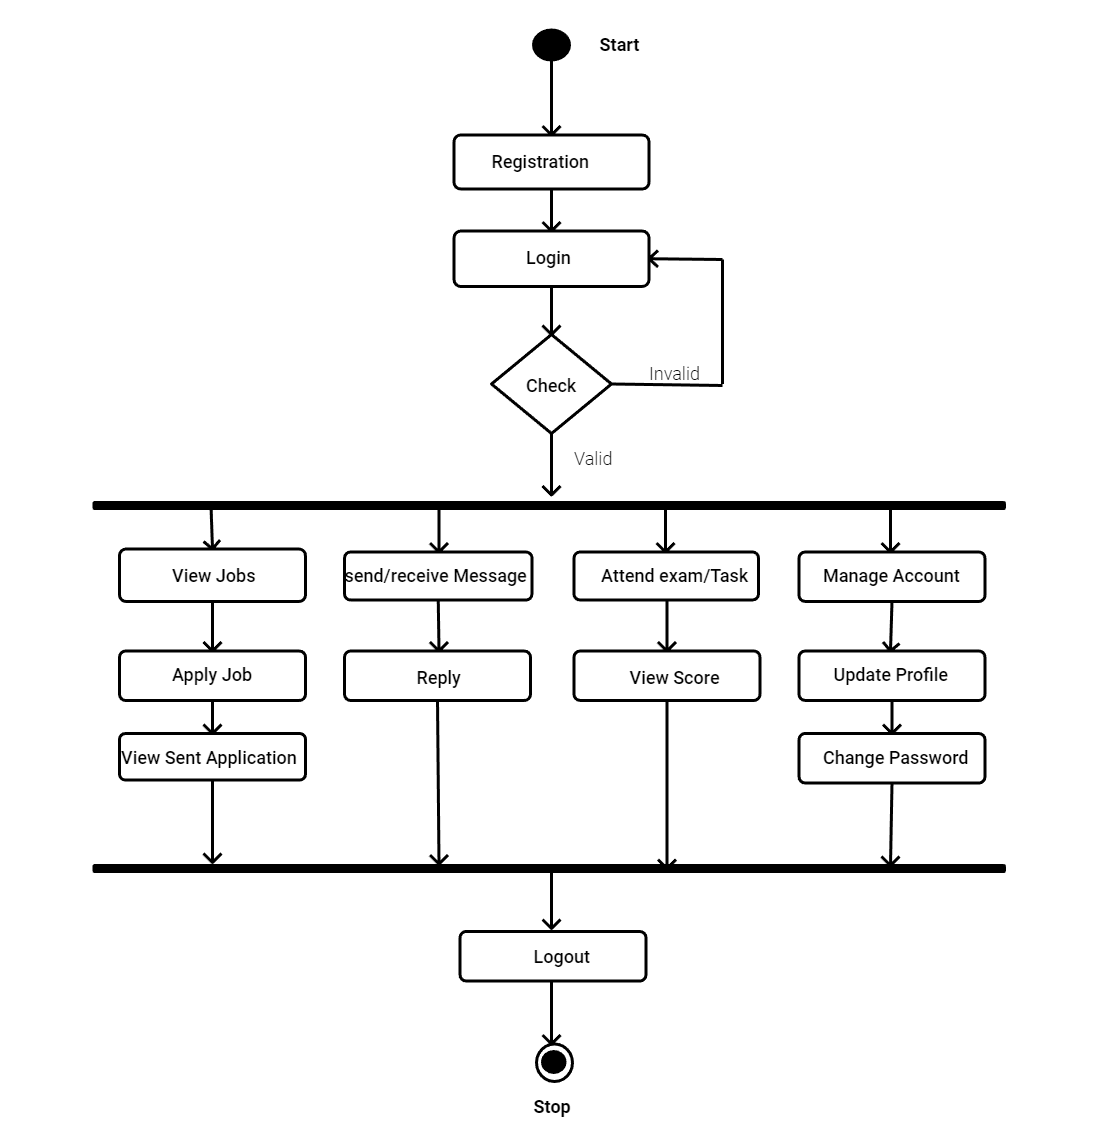
\includegraphics[width=.8\linewidth]{img/useractivity}
	\label{fig:useractivity}
    \caption{User's Activity Diagram}
\end{figure}

\pagebreak
\subitem {\centering \bf - COMPANY}
\vspace*{12pt}
\begin{figure}[bph]
	\centering
	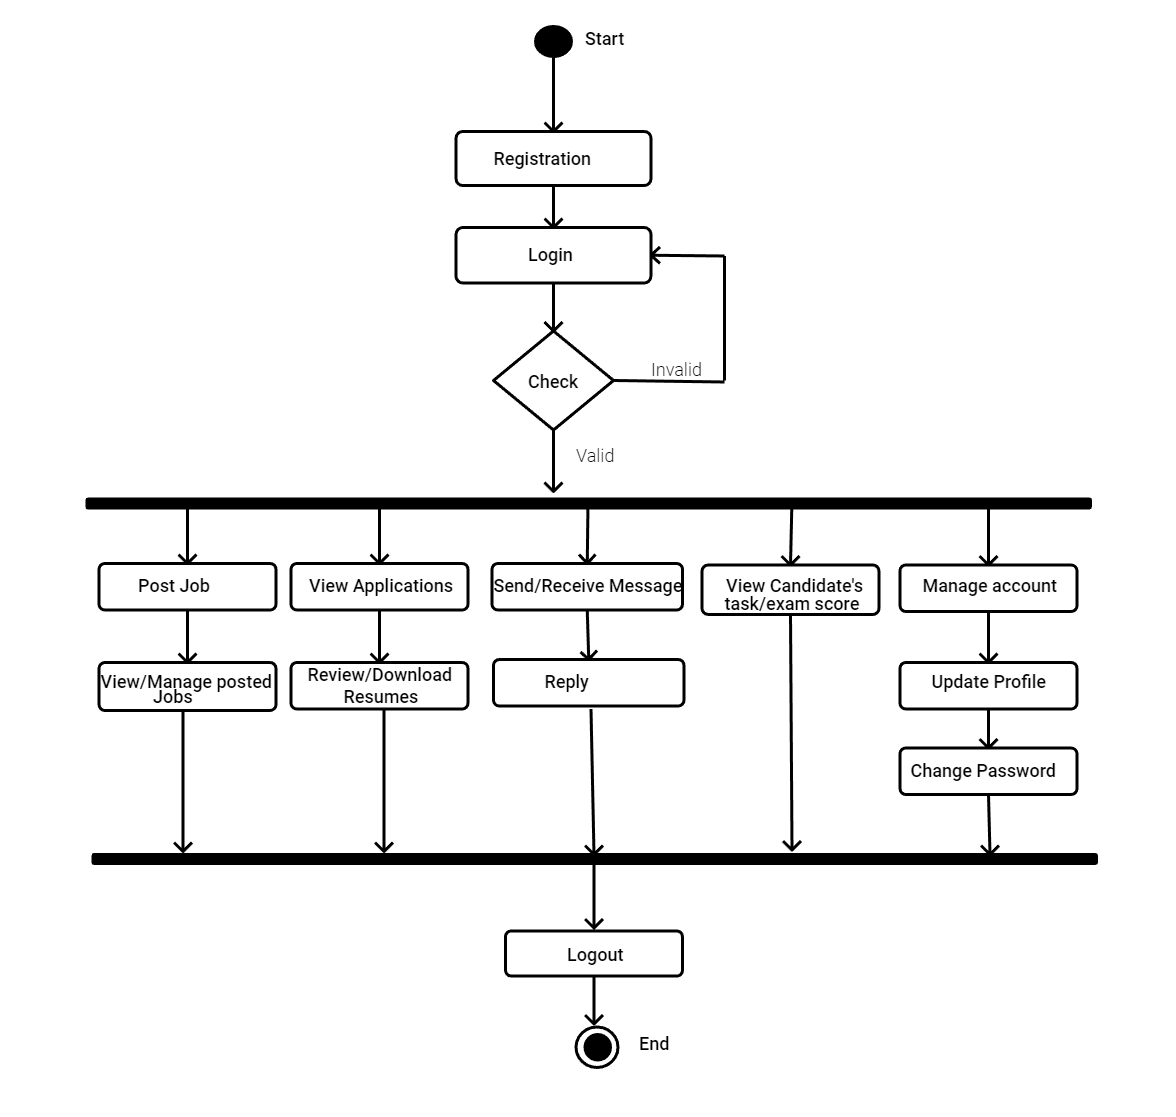
\includegraphics[width=.8\linewidth]{img/cmpnyactivity}
	\label{fig:companyactivity}
	\caption{Company's Activity Diagram}
\end{figure}

\pagebreak

\subitem {\centering \bf - ADMIN}
\vspace*{12pt}
\begin{figure}[bph]
	\centering
	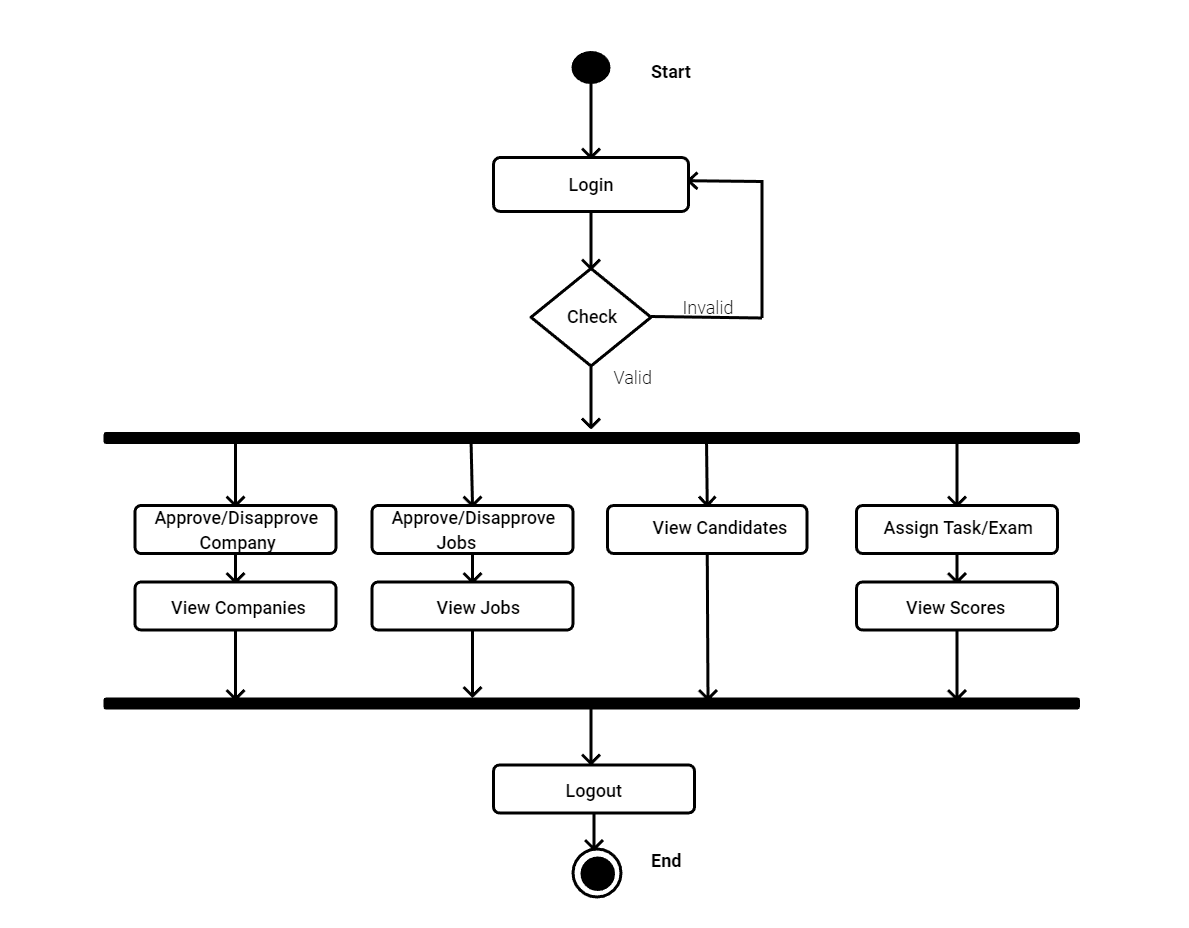
\includegraphics[width=1.1\linewidth]{img/adminactivity}
	\label{fig:adminractivity}
	\caption{Admin's Activity Diagram}
\end{figure}
\pagebreak
\subsection{UseCase Diagrams}

\vspace*{12pt}
\begin{figure}[bph]
	\centering
	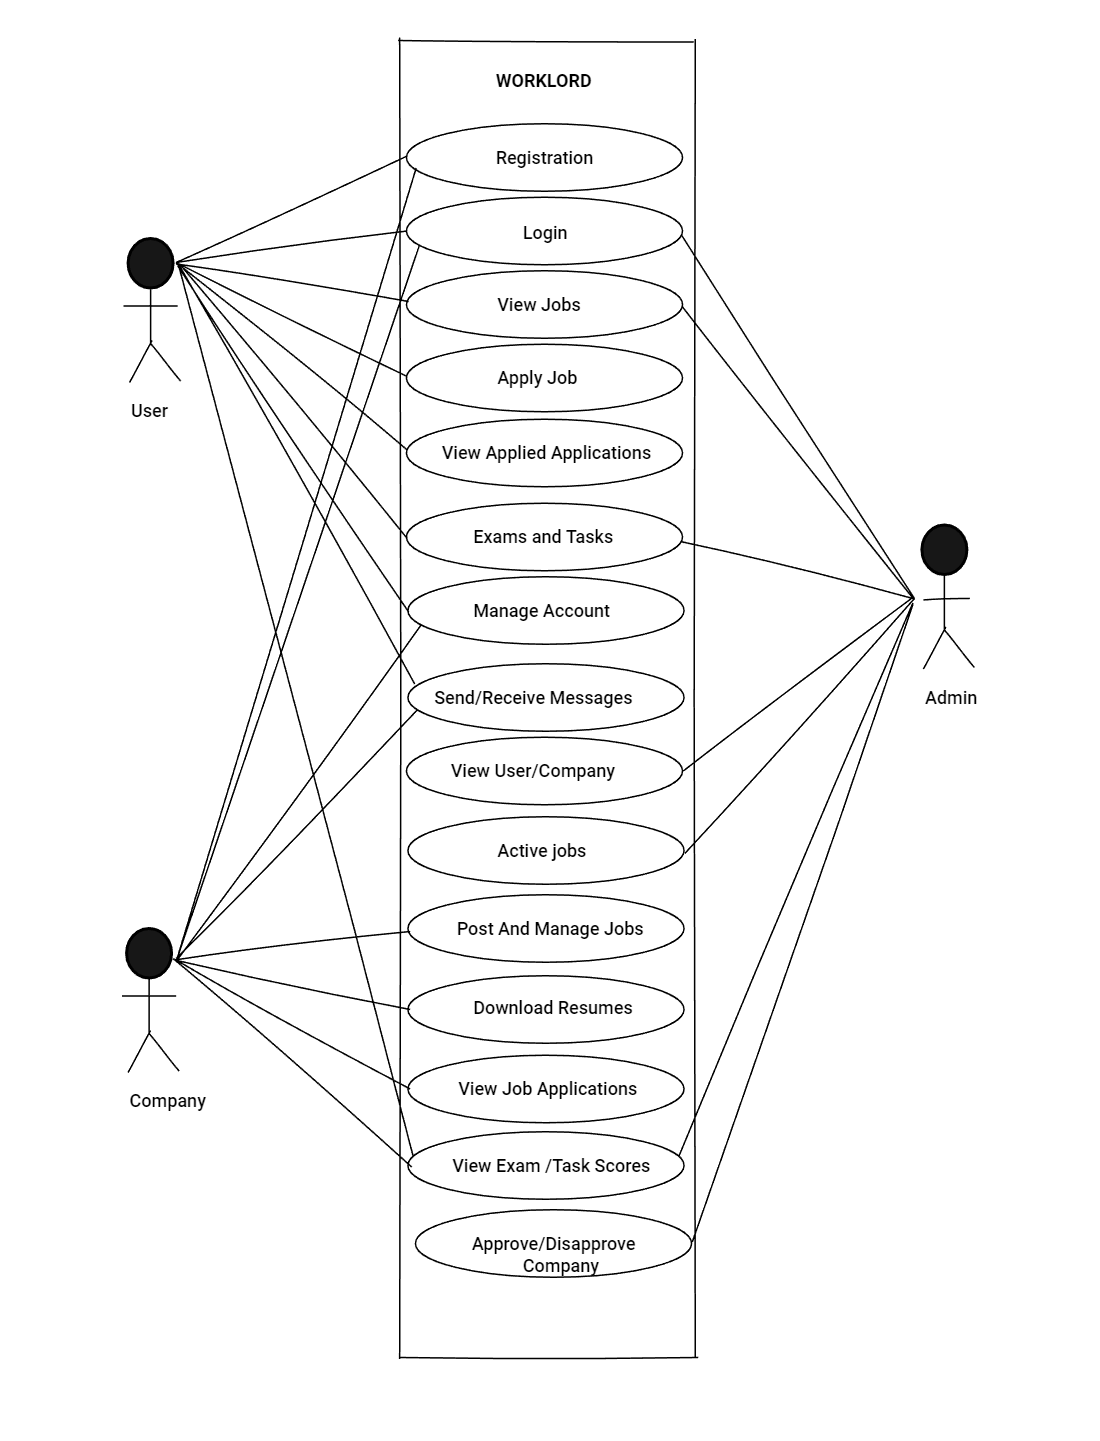
\includegraphics[width=.7\linewidth]{img/use_case_diagram}
	\label{fig:usecasediagram}
	\caption{UseCase Diagram}
\end{figure}
\pagebreak
\section{User Story}
\vspace*{12pt}

\begin{center}
	\begin{tabular}{ | p {1.5 cm} | p {4 cm} | p {3.5 cm} |  p {4.5 cm} | }
		
		\hline 
		User story ID & As a $<$Type of Users$>$ &I want to $<$Perform some task$>$ & So that I can $<$Achieve some goal $>$ \\
		\hline
		1 & Admin/User/Company & Home Page & Go to other activities\\ \hline
		2 & Admin/User/Company & Login & Access the system\\ \hline
		3 & User/Company & Registration & Access the system\\ \hline
		4 & Admin & Approve/Disapprove company & Manage companies\\ \hline
		5 & Admin & View companies & View companies\\ \hline 
		6 & Company & Post jobs & Add Job vaccancies\\ \hline
		7 & Admin & Delete Jobs & Manage jobs\\ \hline
		8 & Admin/User & View jobs & View jobs\\ \hline
		9 & Company & View posted jobs & Manage posted jobs\\ \hline
		10 & Admin & View candidates & View candidates\\ \hline
		11 & User & Apply job & Apply for job\\ \hline
		12 & User & View applications & View applied jobs\\ \hline
		13 & Company & View applications & View job applications\\ \hline
		14 & Company & Download resumes & Download applied candidates resumes\\ \hline
		15 & Admin & Create exams & Create exams\\ \hline
		16 & Admin & Assign tasks & Assign tasks\\ \hline
		17 & User & Attend exam & Attend exam\\ \hline
		18 & User & Attend task & Attend task\\ \hline
		19 & Admin/User/Company & View exam or task scores & Understand knowledge or skills of candidates\\ \hline
		20 & User/Company & Send and Receive Messages & Send/Receive Messages\\ \hline
		21 & User/Company &  Manage account & Update Profile\\ \hline
		22 & User/Company &  Manage account & Change Password\\ \hline

	\end{tabular}
	\captionof{figure}{ User Story}
\end{center}
\pagebreak
\section{ Product Backlog}

\begin{center}
	\begin{tabular}{ | p {1.3 cm} | p {2.3 cm} | p {1 cm} |  p {1.4 cm} |  p {2.5 cm} |  p {1.8 cm} |  p {2.8 cm} | }
	
	\hline
	\centering	\bf USER STORY ID &
	\bf PRIORITY
	(LOW,HIGH,
	MEDIUM)   &
	\bf SIZE &
	\bf SPRINT & 
	\bf STATUS (PLANNED,
	PROGRESSED,
	COMPLETED) &
	\bf RELEASE DATE & 
	\bf RELEASE GOAL \\
	\hline
	
	1& HIGH & 8 & \multirow{5}{*}{1}&Planned   & 15-09-2020 &Login to the system \\ \cline{1-3} \cline{5-7} 
	2& HIGH & 7 &                   &Planned   & 17-09-2020 &Access the system\\ \cline{1-3} \cline{5-7} 
	3& HIGH & 8 &                   &Planned   & 20-09-2020 &Access the account\\ \cline{1-3} \cline{5-7} 
	4& HIGH  & 8 &                   &Planned   & 24-09-2020 &Manage companies\\ \cline{1-3} \cline{5-7}
	5& MEDIUM & 5 &                   &Planned   & 27-09-2020 &View companies\\ \cline{1-3} \cline{5-7} \hline
	6& HIGH & 7 & \multirow{5}{*}{2}&Planned   & 30-09-2020 &Add job vaccanices\\ \cline{1-3} \cline{5-7} 
	7& HIGH & 6 &                   &Planned   & 03-10-2020 &Manage jobs  \\ \cline{1-3} \cline{5-7} 
	8& MEDIUM & 6 &                   &Planned   & 06-10-2020 &View jobs\\ \cline{1-3} \cline{5-7}
	9& HIGH & 10 &                   &Planned   & 09-10-2020 &Manage posted jobs\\ \cline{1-3} \cline{5-7} 
	10& MEDIUM & 6 &                   &Planned   & 11-10-2020 &View Candidates\\ \cline{1-3} \cline{5-7} \hline
	11& HIGH & 9 & \multirow{5}{*}{3}&Planned   & 15-10-2020 &Apply for job\\ \cline{1-3} \cline{5-7} 
	12& MEDIUM & 6 &                   &Planned   & 16-10-2020 &View applied jobs\\ \cline{1-3} \cline{5-7} 
	13& HIGH & 6 &                   &Planned   &17-10-2020 &View job applications\\ \cline{1-3} \cline{5-7} 
	14& MEDIUM & 6 &                   &Planned   & 19-10-2020 &Download applied candidates resumes  \\ \cline{1-3} \cline{5-7}
	15& HIGH & 10 &                   &Planned   & 23-10-2020 &Create exams\\ \cline{1-3} \cline{5-7}  \hline             
\end{tabular}
\end{center}
\pagebreak

\begin{center}
	\begin{tabular}{ | p {1.3 cm} | p {2.3 cm} | p {1 cm} |  p {1.4 cm} |  p {2.5 cm} |  p {1.8 cm} |  p {2.8 cm} | }
		
		\hline
		\centering	\bf USER STORY ID &
		\bf PRIORITY
		(LOW,HIGH,
		MEDIUM)   &
		\bf SIZE &
		\bf SPRINT & 
		\bf STATUS (PLANNED,
		PROGRESSED,
		COMPLETED) &
		\bf RELEASE DATE & 
		\bf RELEASE GOAL \\
		\hline
		16& MEDIUM & 7 &3 &Planned   & 26-10-2020 &Assign task\\ \cline{1-3} \cline{5-7}\hline
		17& HIGH & 8 &   \multirow{6}{*}{4}  &Planned   & 31-10-2020 &Attend exam\\ \cline{1-3} \cline{5-7} 
		18& HIGH & 8 &                   &Planned   & 01-11-2020 &Attend task\\ \cline{1-3} \cline{5-7} 
		19& MEDIUM & 7 &                   &Planned   & 02-11-2020 &Understand knowledge or skills of candidates\\ \cline{1-3} \cline{5-7}
		20& MEDIUM & 6 &                   &Planned   & 05-11-2020 &Send/Receive Messages\\ \cline{1-3} \cline{5-7}
		21& MEDIUM & 7 &                   &Planned   & 07-11-2020 &Update profile \\ \cline{1-3} \cline{5-7}
		22& MEDIUM & 7 &                   &Planned   & 08-11-2020 & Change password\\ \cline{1-3} \cline{5-7} \hline   
	\end{tabular}
\captionof{figure}{ Product Backlog}
\end{center}
\pagebreak
\section{Project Plan}
\vspace*{12pt}
\begin{center}
	\begin{tabular}{ | p {1.5 cm} | p {2.5 cm} | p {2 cm} |  p {2 cm} |  p {1 cm} |  p {2.2 cm} |}		
		\hline
		\centering	\bf USER STORY ID &
		\bf TASK   
		NAME     &
		\bf START
		DATE &
		\bf END
		DATE & 
		\bf DAYS &
		\bf STATUS ( TO 
		BE FILLED BY 
		SCRUM MASTER ) \\
		\hline
		
		1&\multirow{5}{*}{SPRINT 1}& 14-09-2020  & 15-09-2020  & 2 &  \\ \cline{1-1} \cline{3-6}
		2&						   & 16-09-2020  & 17-09-2020  & 2 &  \\ \cline{1-1} \cline{3-6}
		3&                         & 18-09-2020  & 20-09-2020  & 3 &  \\ \cline{1-1} \cline{3-6}
		4&                         & 21-09-2020 & 24-09-2020  & 4  &  \\ \cline{1-1} \cline{3-6}
		5&                         & 25-09-2020  & 27-09-2020  & 3 &  \\ \cline{1-1} \cline{3-6}\hline
		6&\multirow{5}{*}{SPRINT 2}& 29-09-2020  &  30-09-2020 & 2  &  \\ \cline{1-1} \cline{3-6}
		7&						   & 01-10-2020 & 03-10-2020  & 3 &  \\ \cline{1-1} \cline{3-6}
		8&						   & 04-10-2020  & 06-10-2020 & 3 &  \\ \cline{1-1} \cline{3-6} 
		9&						   & 07-10-2020  & 09-10-2020  & 3 &  \\ \cline{1-1} \cline{3-6}
		10&						   & 10-10-2020  & 11-10-2020  & 2 &  \\ \cline{1-1} \cline{3-6}\hline
		11&\multirow{5}{*}{SPRINT 3}&  13-10-2020 & 15-10-2020  & 3 &  \\ \cline{1-1} \cline{3-6}
		12&						   & 16-10-2020  &  16-10-2020 & 1 &  \\ \cline{1-1} \cline{3-6}
		13&						   &  17-10-2020 & 17-10-2020  & 1 &  \\ \cline{1-1} \cline{3-6} 
		14&						   &  18-10-2020 & 19-10-2020  & 2 &  \\ \cline{1-1} \cline{3-6}
		15&						   &  20-10-2020 &  23-10-2020 & 4 &  \\ \cline{1-1} \cline{3-6}
		16&						   &  24-10-2020 &  26-10-2020 & 3 &  \\ \cline{1-1} \cline{3-6}\hline
		17&\multirow{5}{*}{SPRINT 4}& 28-10-2020  &  31-10-2020 & 4 &  \\ \cline{1-1} \cline{3-6}
		18&						   &  01-11-2020 & 01-11-2020  & 1 &  \\ \cline{1-1} \cline{3-6} 
		19&						   & 02-11-2020  & 02-11-2020  & 1 &  \\ \cline{1-1} \cline{3-6}
		20&						   & 03-11-2020  & 04-11-2020  & 2 &  \\ \cline{1-1} \cline{3-6}
		21&						   &  05-11-2020 & 06-11-2020  & 2 &  \\ \cline{1-1} \cline{3-6}
		22&						   & 07-07-2020  & 08-07-2020  & 2 &  \\ \cline{1-1} \cline{3-6}\hline
		
		
	\end{tabular}
\captionof{figure}{ Project Plan}
\end{center}
\pagebreak
\section{Sprint Backlog Planned}
\subsection {Sprint 1}
\begin{figure}[bph]
	\centering
	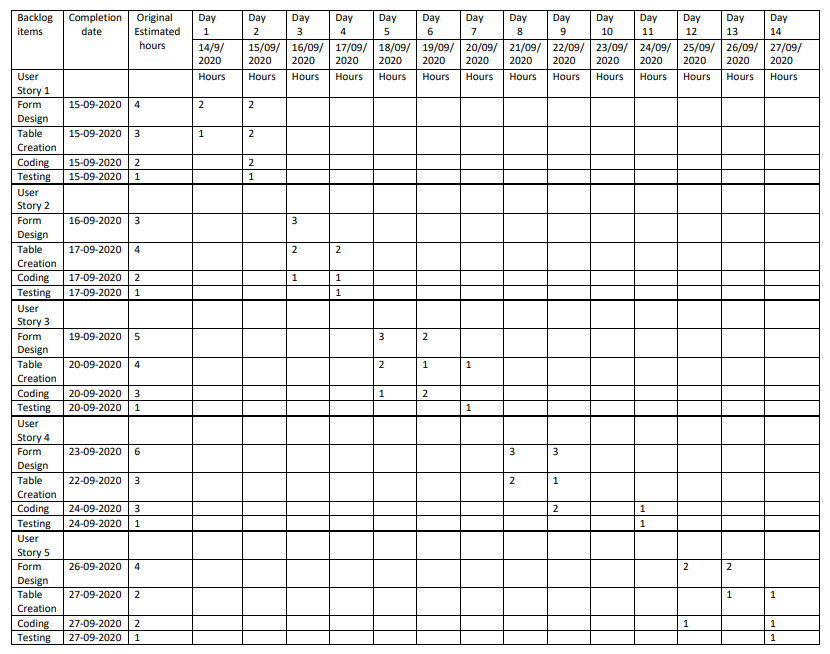
\includegraphics[width=1.1\linewidth]{img/sprint1}
	\caption{Login}
\end{figure}
\pagebreak

\section{Database Design}
\subsection{Admin Table}
This Table stores login details of Admins

\begin{center}
	\begin{tabular} { | p {1 cm} | p {3 cm} | p {3 cm} |  p {3 cm} |  p {4 cm} | }
		
		\hline
		\centering	\bf No. &
		\bf FIELD NAME &
		\bf TYPE &
		\bf CONSTRAINTS & 
		\bf DESCRIPTION \\
		\hline
		
		
		\centering	1 &adminid & INT(11) & PRIMARY KEY & Admin's ID\\ \hline
		\centering	2 &username & VARCHAR(50) & UNIQUE & Admin's Username\\ \hline
		\centering	3 &password & VARCHAR(50) & NOTNULL & Admin's Password\\ \hline
		\centering	4 &email & VARCHAR(20) & UNIQUE & Admin's Email\\ \hline
	\end{tabular}
	\vspace*{12pt}
\captionof{table}{ Admin Table}
\end{center}


\subsection{Company Table}
This Table stores Login and Company details
\begin{center}
	\begin{tabular} { | p {1 cm} | p {3.5 cm} | p {3 cm} |  p {3 cm} |  p {4 cm} | }
		
		\hline
		\centering	\bf No. &
		\bf FIELD NAME &
		\bf TYPE &
		\bf CONSTRAINTS & 
		\bf DESCRIPTION \\
		\hline
		
		1 & companyid & INT(11) & PRIMARY KEY & Company ID\\ \hline
		2 & companyname & VARCHAR(50) & NOTNULL & Company Name\\ \hline
		3 & email & VARCHAR(20) & UNIQUE & Company Email\\ \hline
		4 & password & VARCHAR(20) & NOTNULL & Company Password\\ \hline
		5 & country & VARCHAR(50) & NOTNULL & Company Country\\ \hline
		6 & city & VARCHAR(50) & NOTNULL & Company City\\ \hline
		7 & state & VARCHAR(10) & NOTNULL & Company State\\ \hline
		8 & contactno & VARCHAR(50) & NOTNULL & Company Phone Number\\ \hline
		9 & website & VARCHAR(50) & NOTNULL & Company Website\\ \hline
		10 & aboutme & VARCHAR(100) & NOTNULL & About Company\\ \hline
		11 & logo & VARCHAR(100) & NOTNULL & Company Logo Name\\ \hline
		
		
	\end{tabular}

\captionof{table}{ Company Table}
\end{center}

\pagebreak

\subsection{User Table}
This Table stores Login details and User details
\begin{center}
	\begin{tabular} { | p {1 cm} | p {3.5 cm} | p {3 cm} |  p {3 cm} |  p {4 cm} | }
		
		\hline
		\centering	\bf No. &
		\bf FIELD NAME &
		\bf TYPE &
		\bf CONSTRAINTS & 
		\bf DESCRIPTION \\
		\hline
		
		
		1 & userid & INT(11) & PRIMARY KEY & User's ID\\ \hline
		2 & firstname & VARCHAR(50) & NOTNULL & User's Firstname\\ \hline
		3 & lastname & VARCHAR(50) & NOTNULL & User's Lastname\\ \hline
		4 & email & VARCHAR(20) & UNIQUE &User's Email\\ \hline
		5 & password & VARCHAR(20) & NOTNULL & User's Password\\ \hline
		6 & address & VARCHAR(50) & NOTNULL & User's Address\\ \hline
		7 & city & VARCHAR(50) & NOTNULL & User's City\\ \hline
		8 & state & VARCHAR(10) & NOTNULL & User's State\\ \hline
		9 & contactno & VARCHAR(50) & NOTNULL & User's Phone Number\\ \hline
		10 & qualifications & VARCHAR(50) & NOTNULL & User's Qualifications\\ \hline
		11 & stream & VARCHAR(20) & NOTNULL & User's Course\\ \hline
		12 & passingyear & VARCHAR(10) & NOTNULL & User's Year Of Passing\\ \hline
		13 & dob & DATE & NOTNULL & User's Date Of Birth\\ \hline
		14 & age & VARCHAR(50) & NOTNULL & User's Age\\ \hline
		15 & designation & VARCHAR(50) & NOTNULL & User's Preferred Designation\\ \hline
		16 & aboutme & VARCHAR(100) & NOTNULL & About User\\ \hline
		17 & skills & VARCHAR(50) & NOTNULL & User's Skills\\ \hline
		18 & resume & VARCHAR(100) & NOTNULL & User's Resume Name\\ \hline
		
		
	\end{tabular}
	\vspace*{12pt}
\captionof{table}{ User Table}
\end{center}
\pagebreak

\subsection{Job Post Table}
This Table stores Job Posts provided by the Companies
\begin{center}
	\begin{tabular} { | p {.5 cm} | p {4 cm} | p {3 cm} |  p {3 cm} |  p {4 cm} | }
		
		\hline
		\centering	\bf No. &
		\bf FIELD NAME &
		\bf TYPE &
		\bf CONSTRAINTS & 
		\bf DESCRIPTION \\
		\hline
		
		
		1 & postid & INT(11) & PRIMARY KEY & Post ID\\ \hline
		2 & companyid & INT(11) & FOREIGN KEY & Company ID\\ \hline
		3 & jobtitle & VARCHAR(20) & NOTNULL & Job Title\\ \hline
		4 & description & VARCHAR(20) & NOTNULL & About Job\\ \hline
		5 & minimumsalary & VARCHAR(50) & NOTNULL & Minimum Salary\\ \hline
		6 & maximumsalary & VARCHAR(50) & NOTNULL & Maximum Salary\\ \hline
		7 & experience & VARCHAR(10) & NOTNULL & Experience State\\ \hline
		8 & qualifications & VARCHAR(50) & NOTNULL & Job Qualifications\\ \hline
		
		
	\end{tabular}
	\vspace*{12pt}
	\captionof{table}{ Job Post Table}
\end{center}

\subsection{Job Apply Table}
This Table stores Applied User's details and status of Application
\begin{center}
	\begin{tabular} { | p {1 cm} | p {3 cm} | p {3 cm} |  p {3 cm} |  p {4 cm} | }
		
		\hline
		\centering	\bf No. &
		\bf FIELD NAME &
		\bf TYPE &
		\bf CONSTRAINTS & 
		\bf DESCRIPTION \\
		\hline
		
		1 & applyid & INT(11) & PRIMARY KEY & Job Application Apply ID\\ \hline
		2 & jobpostid & INT(11) & NOTNULL & Job Post ID\\ \hline
		4 & userid & INT(11) & NOTNULL & User's ID\\ \hline
		5 & status & INT(11) & NOTNULL & Application Status\\ \hline
		
	\end{tabular}
	\vspace*{12pt}
	\captionof{table}{ Job Apply Table}
\end{center}

\pagebreak

\subsection{Exams Table}
This Table stores Exam details
\begin{center}
	\begin{tabular} { | p {1 cm} | p {3 cm} | p {3 cm} |  p {3 cm} |  p {4 cm} | }
		
		\hline
		\centering	\bf No. &
		\bf FIELD NAME &
		\bf TYPE &
		\bf CONSTRAINTS & 
		\bf DESCRIPTION \\
		\hline
		
		1 & examid & INT(11) & PRIMARY KEY & Exam ID\\ \hline
		2 & category & VARCHAR(50) & NOTNULL & Exam Category\\ \hline
		3 & examname & VARCHAR(50) & NOTNULL & Exam Name\\ \hline
		4 & date & DATE & NOTNULL & Exam Date\\ \hline
		5 & passmark & INT(10) & NOTNULL & Exam Passmark\\ \hline
		6 & duration & TIME & NOTNULL & Exam Duration\\ \hline
		7 & terms & VARCHAR(50) & NOTNULL & Exam Terms\\ \hline	
		
	\end{tabular}
	\vspace*{12pt}
	\captionof{table}{ Exams Table}
\end{center}

\subsection{Exam Questions Table}
This Table stores Questions for each Exams
\begin{center}
	\begin{tabular} { | p {1 cm} | p {3 cm} | p {3 cm} |  p {3 cm} |  p {4 cm} | }
		
		\hline
		\centering	\bf No. &
		\bf FIELD NAME &
		\bf TYPE &
		\bf CONSTRAINTS & 
		\bf DESCRIPTION \\
		\hline
		
		
		1 & questionid & INT(11) & PRIMARY KEY & Question ID\\ \hline
		2 & examid & VARCHAR(50) & FOREIGN KEY & Exam ID\\ \hline
		3 & category & VARCHAR(50) & NOTNULL & Question Category\\ \hline
		4 & question & LONGTEXT & NOTNULL & Question \\ \hline
		5 & option1 & VARCHAR(50) & NOTNULL & Question Option 1\\ \hline 
		6 & option2 & VARCHAR(50) & NOTNULL &Question Option 2 \\ \hline
		7 & option3 & VARCHAR(50) & NOTNULL & Question Option 3 \\ \hline
		8 & option4 & VARCHAR(50) & NOTNULL & Question Option 4 \\ \hline
		9 & answer & VARCHAR(50) & NOTNULL & Question Answer  \\ \hline
		
	\end{tabular}
	\vspace*{12pt}
	\captionof{table}{ Exam Questions Table}
\end{center}

\pagebreak

\subsection{Exam Score Table}
This Table stores Applied User's details and status of Application
\begin{center}
	\begin{tabular} { | p {1 cm} | p {3 cm} | p {3 cm} |  p {3 cm} |  p {4 cm} | }
		
		\hline
		\centering	\bf No. &
		\bf FIELD NAME &
		\bf TYPE &
		\bf CONSTRAINTS & 
		\bf DESCRIPTION \\
		\hline
		
		
		1 & scoreid & INT(11) & PRIMARY KEY & Record ID\\ \hline
		2 & userid & VARCHAR(50) & FOREIGN KEY & User's ID\\ \hline
		3 & examname & VARCHAR(20) & UNIQUE & Exam Name\\ \hline
		4 & score & VARCHAR(50) & NOTNULL & User's Score\\ \hline
		5 & date & VARCHAR(50) & NOTNULL & Exam Date\\ \hline
		
		
	\end{tabular}
	\captionof{table}{ Exam Score Table}
\end{center}


\subsection{Task Table}
This Table stores Task Details
\begin{center}
	\begin{tabular} { | p {1 cm} | p {3 cm} | p {3 cm} |  p {3 cm} |  p {4 cm} | }
		
		\hline
		\centering	\bf No. &
		\bf FIELD NAME &
		\bf TYPE &
		\bf CONSTRAINTS & 
		\bf DESCRIPTION \\
		\hline
		
		1 & taskid & INT(11) & PRIMARY KEY & Task ID\\ \hline
		2 & category & VARCHAR(50) & NOTNULL & Task Category\\ \hline
		3 & taskdetails & LONGTEXT & NOTNULL & Task Details\\ \hline
		
	\end{tabular}
	\captionof{table}{ Task Table}
\end{center}
\subsection{Task Submit Table}
This Table stores Submitted task details,Status and Scores

\begin{center}
	\begin{tabular}[ht] { | p {1 cm} | p {3 cm} | p {3 cm} |  p {3 cm} |  p {4 cm} | }
		
		\hline
		\centering	\bf No. &
		\bf FIELD NAME &
		\bf TYPE &
		\bf CONSTRAINTS & 
		\bf DESCRIPTION \\
		\hline
		
		1 & taskid & INT(11) & PRIMARY KEY & Task ID\\ \hline
		2 & userid & INT(11) & FOREIGN KEY & Candidate ID\\ \hline
		3 & tasksubmitstatus & INT(10) & NOTNULL & Task Submit Status\\ \hline
		4 & taskreviewstatus & INT(10) & NOTNULL & Task Review Status\\ \hline
		5 & tasklink & VARCHAR(100) & NOTNULL & Task Github Link\\ \hline
		6 & taskscore & INT(10) & NOTNULL & Task Status\\ \hline
		
	\end{tabular}
	\captionof{table}{ Tasks Submit Table}
\end{center}

\pagebreak

\subsection{MailBox}
This Table stores Mail Send to User/Company

\begin{center}
	\begin{tabular}[ht] { | p {1 cm} | p {3 cm} | p {3 cm} |  p {3 cm} |  p {4 cm} | }
		
		\hline
		\centering	\bf No. &
		\bf FIELD NAME &
		\bf TYPE &
		\bf CONSTRAINTS & 
		\bf DESCRIPTION \\
		\hline
		
		1 & idmailbox & INT(11) & PRIMARY KEY & Mail ID\\ \hline
		2 & idfromuser & INT(11) & FOREIGN KEY & ID of user send message\\ \hline
		3 & fromuser & VARCHAR(10) & NOTNULL & Type of user who send\\ \hline
		4 & idtouser & INT(10) & NOTNULL & The id of user to be send\\ \hline
		5 & subject & VARCHAR(100) & NOTNULL & Message subject\\ \hline
		6 & message & INT(10) & NOTNULL & Message \\ \hline
		6 & date & DATE & NOTNULL & Date of message creation\\ \hline
		
	\end{tabular}
	\captionof{table}{ Tasks Submit Table}
\end{center}

\pagebreak
\section{User Interface Design}
\subsection {Homepage}
Homepage of Worklord Website
\begin{figure}[bph]
	\centering
	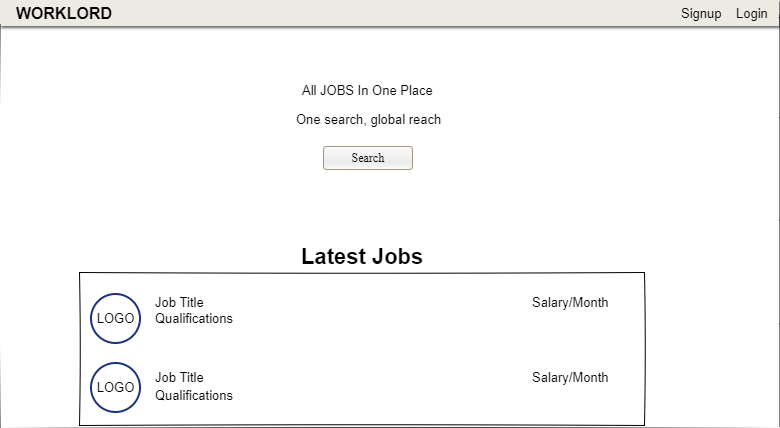
\includegraphics[width=.6\linewidth]{img/homepage}
	\caption{Homepage}
\end{figure}
\subsection {Login}
Login Page for admin,company and users
\begin{figure}[bph]
	\centering
	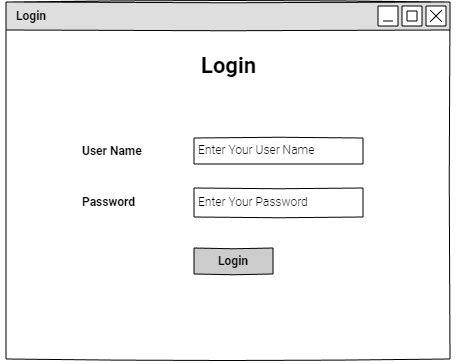
\includegraphics[width=.4\linewidth]{img/login}
	\caption{Login}
\end{figure}
\pagebreak

\subsection {Job Search}
Helps to Search Available Jobs in the website
\begin{figure}[bph]
	\centering
	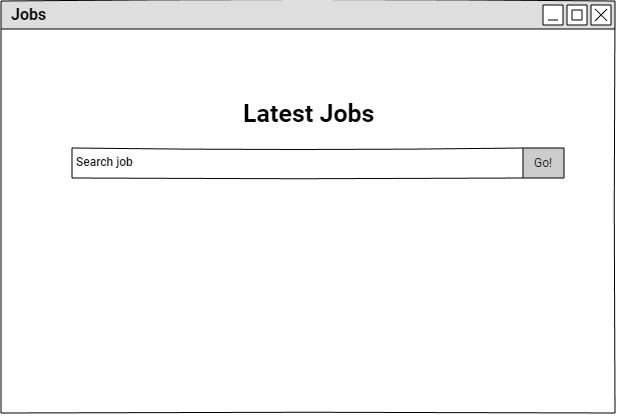
\includegraphics[width=.65\linewidth]{img/searchjob}
	\caption{Job Search}
\end{figure}
\subsection {Jobs}
Job Details
\begin{figure}[bph]
	\centering
	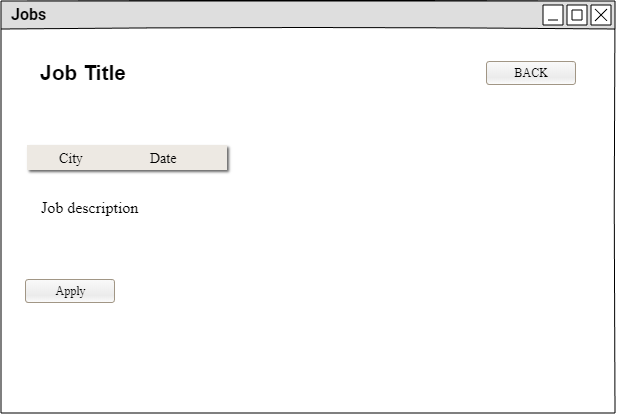
\includegraphics[width=.6\linewidth]{img/searchjobapply}
	\caption{Jobs}
\end{figure}
\pagebreak

\subsection {Mailbox}
View messages from User/Company and Compose messages to User/Company
\begin{figure}[bph]
	\centering
	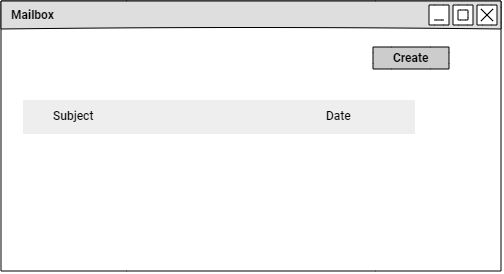
\includegraphics[width=.7\linewidth]{img/notification}
	\caption{MailBox}
\end{figure}


\subsection {View Mailbox}
View messages from User/Company and Reply to those messages
\begin{figure}[bph]
	\centering
	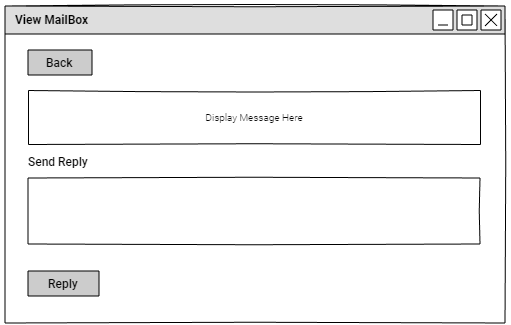
\includegraphics[width=.7\linewidth]{img/view_notifctn}
	\caption{View MailBox}
\end{figure}
\pagebreak

\subsection {Compose Message}
Compose Messages to User or Company (Shows users Applied for Jobs)
\begin{figure}[bph]
	\centering
	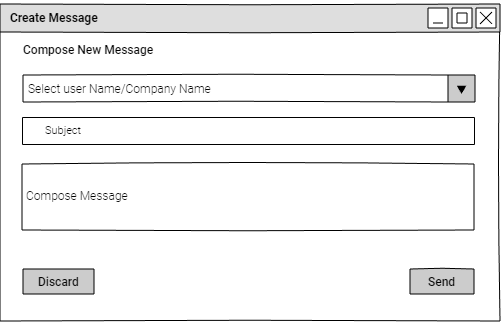
\includegraphics[width=.5\linewidth]{img/create_msg}
	\caption{Compose Message}
\end{figure}
\addcontentsline{toc}{section}{ - User}
\subsection {User Registration}
Registration form for User
\begin{figure}[bph]
	\centering
	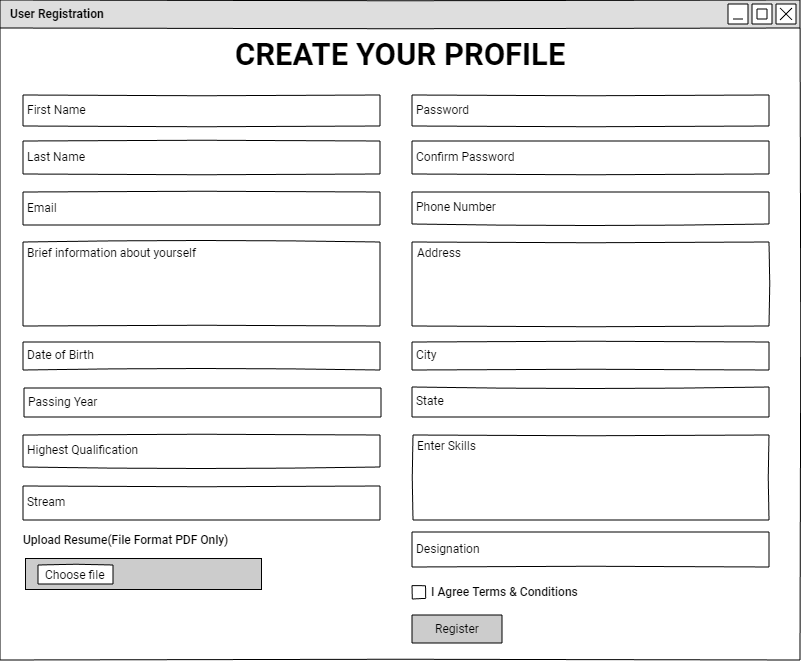
\includegraphics[width=.6\linewidth ]{img/user/user_registration}
	\caption{User Registration}
\end{figure}
\pagebreak

\subsection {Dashboard}
Dashboard for Users, Shows available functions for user
\begin{figure}[bph]
	\centering
	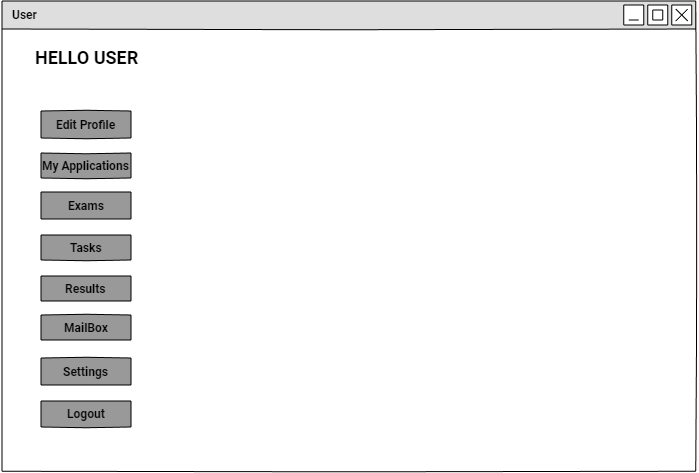
\includegraphics[width=.8\linewidth]{img/user/userhompage}
	\caption{Dashboard}
\end{figure}
\subsection {My Applications}
Applied Job's Details and Status
\begin{figure}[bph]
	\centering
	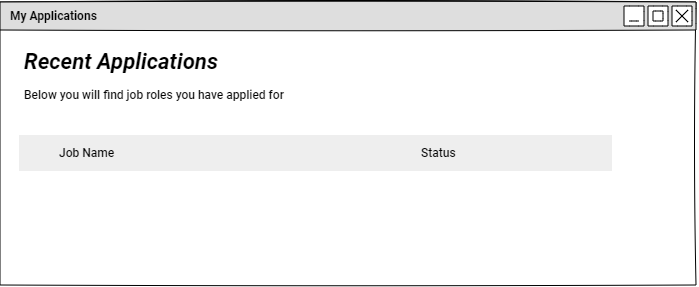
\includegraphics[width=.7\linewidth]{img/user/useraplictns}
	\caption{My Applications}
\end{figure}
\pagebreak
\subsection {Update Profile}
Update User's Details and Resume
\begin{figure}[bph]
	\centering
	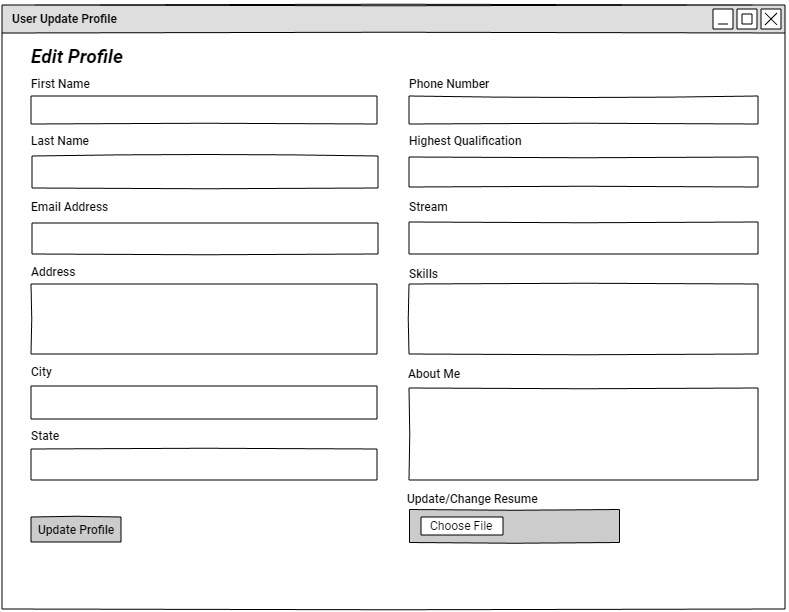
\includegraphics[width=.7\linewidth ]{img/user/userupdate}
	\caption{Update Profile}
\end{figure}

\subsection {Exams}
Attend Exams and View scores
\begin{figure}[bph]
	\centering
	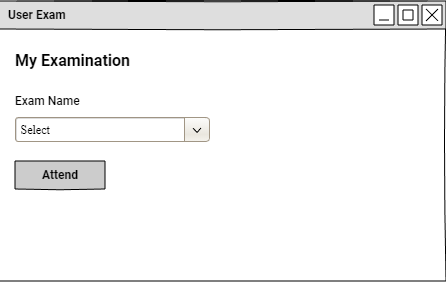
\includegraphics[width=.4\linewidth]{img/user/userexm}
		\caption{Exams}
\end{figure}
\pagebreak

\subsection {Tasks}
Attend Tasks
\begin{figure}[bph]
	\centering
	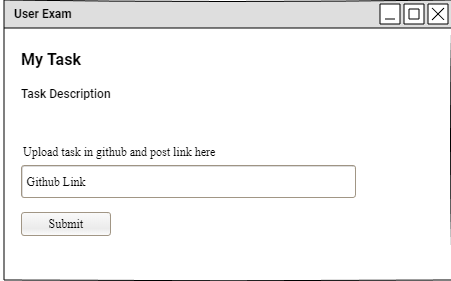
\includegraphics[width=.6\linewidth ]{img/user/usertasks}
\caption{Tasks}
\end{figure}

\subsection {Results}
View Scores for Task and Exams
\begin{figure}[bph]
	\centering
	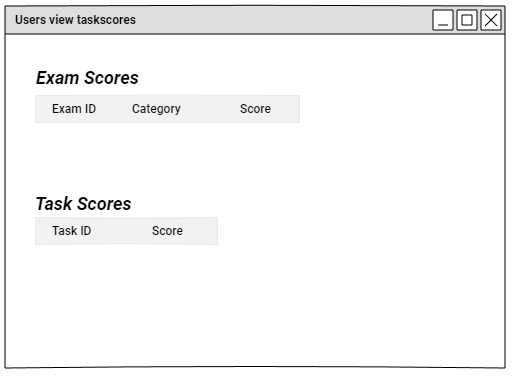
\includegraphics[width=.6\linewidth ]{img/user/userviewscr}
\caption{Results}
\end{figure}
\pagebreak

\pagebreak
\subsection {Settings}
Change Password or Delete Account
\begin{figure}[bph]
	\centering
	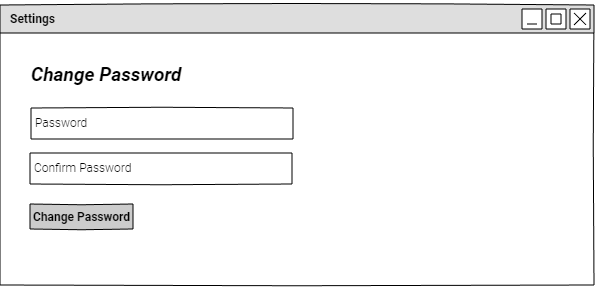
\includegraphics[width=.6\linewidth ]{img/user/userstings}
	\caption{Settings}
\end{figure}

\addcontentsline{toc}{section}{ - Company}
\subsection {Company Registration}
Registration form for company
\begin{figure}[bph]
	\centering
	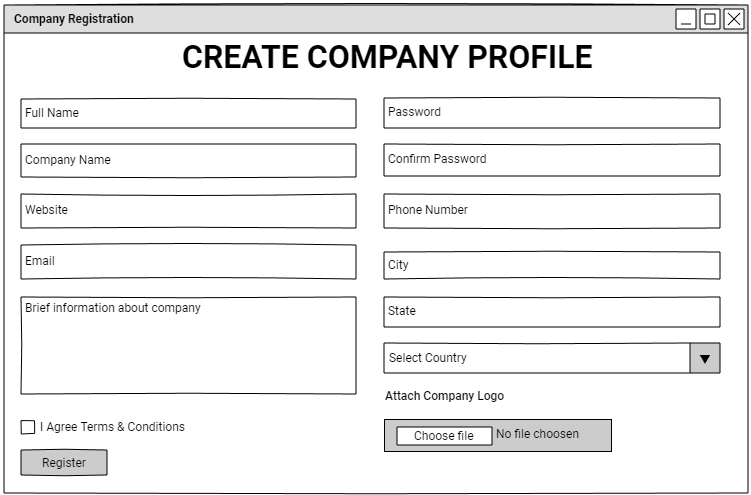
\includegraphics[width=.8\linewidth ]{img/company/company_registration}
	\caption{Company Registration}
\end{figure}
\pagebreak
\subsection {Dashboard}
Dashboard for company
\begin{figure}[bph]
	\centering
	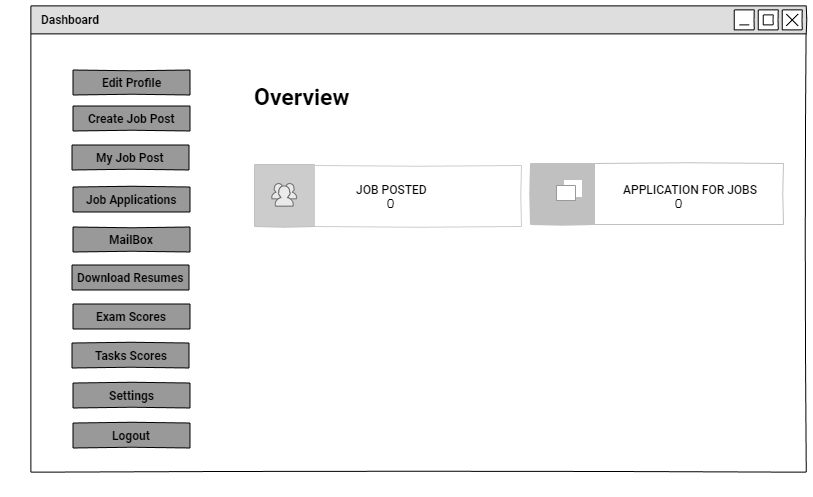
\includegraphics[width=1\linewidth]{img/company/company_home_page}
	\caption{Dashboard}
\end{figure}

\pagebreak
\subsection {Edit Profile}
Edit Company details
\begin{figure}[bph]
	\centering
	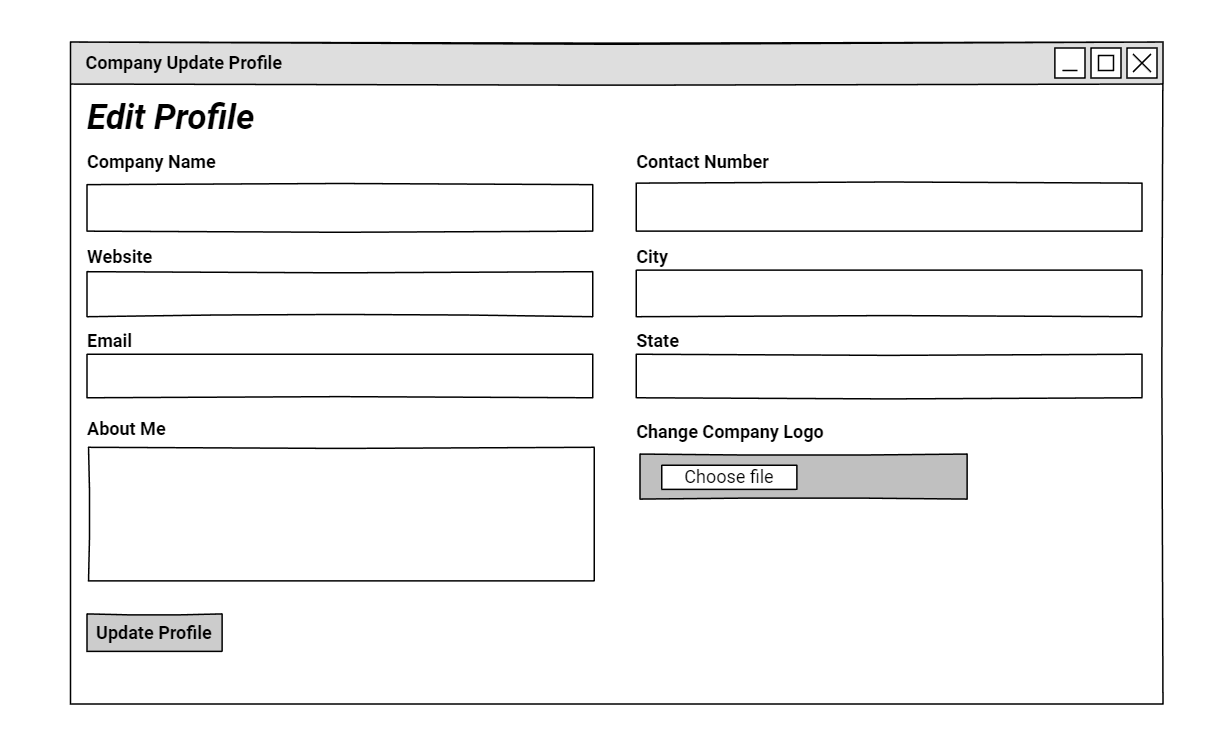
\includegraphics[width=.6\linewidth]{img/company/cmpnyprflupdt}
		\caption{Edit Profile}
\end{figure}

\subsection {Create Job Post}
Create New Job Posts with Details
\begin{figure}[bph]
	\centering
	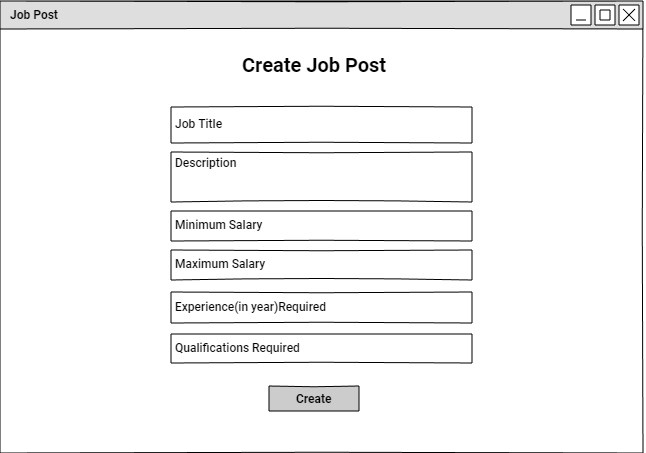
\includegraphics[width=.6\linewidth]{img/company/createpostjob}
	\caption{Create Job Post}
\end{figure}
\pagebreak
\subsection {Job Posts}
View posted Jobs by Company
\begin{figure}[bph]
	\centering
	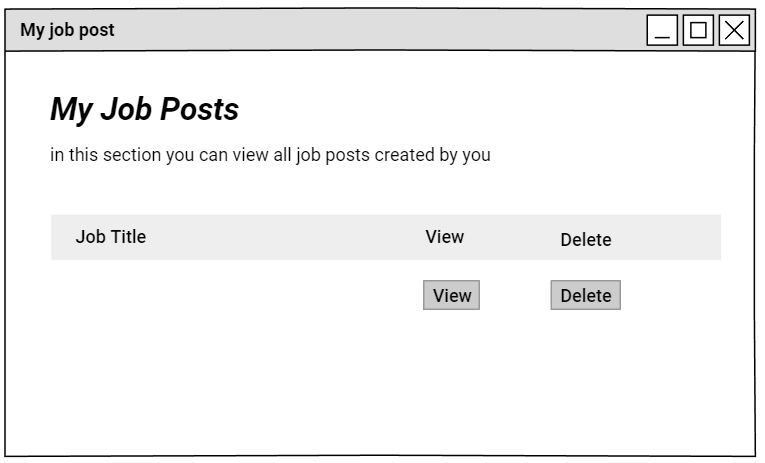
\includegraphics[width=.6\linewidth]{img/company/postedjobs}
	\caption{Job Posts}
\end{figure}

\subsection {Job Applications}
View Job Post Applications from Users and Review
\begin{figure}[bph]
	\centering
	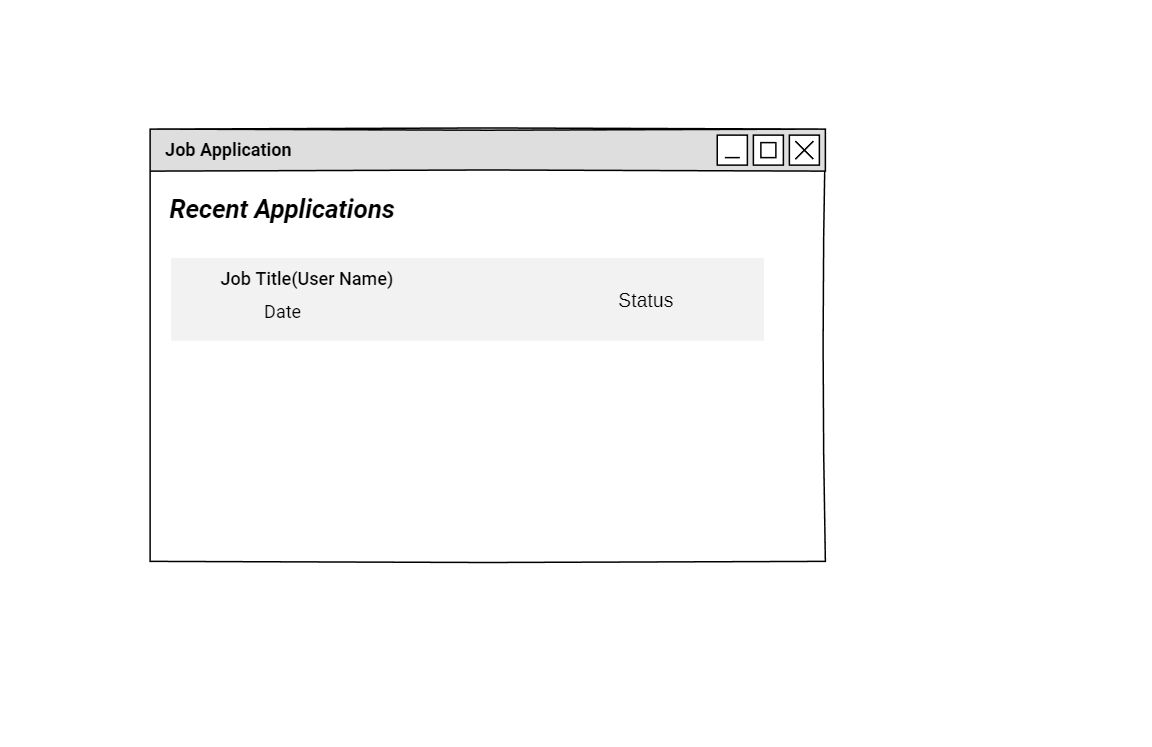
\includegraphics[width=.7\linewidth]{img/company/jobapltns}
	\caption{Job Applications}
\end{figure}
\pagebreak

\subsection {Download Resumes}
Download Resumes of Applied Users for Company's Job Posts
\begin{figure}[bph]
	\centering
	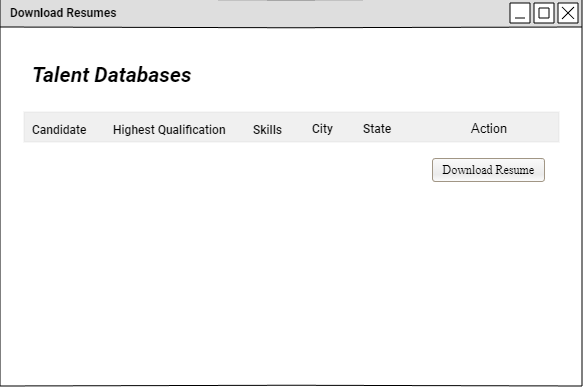
\includegraphics[width=.7\linewidth]{img/company/dwnldresm}
	\caption{Download Resume}
\end{figure}

\subsection {Exam Scores}
Exam Scores of Applied Users for Company's Job Posts
\begin{figure}[bph]
	\centering
	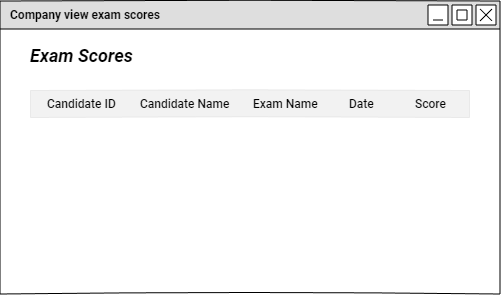
\includegraphics[width=.6\linewidth]{img/company/cmpnyviewexmscr}
	\caption{Exam Scores}
\end{figure}
\pagebreak
\subsection {Task Scores}
Task Scores of Applied Users for Company's Job Posts
\begin{figure}[bph]
	\centering
	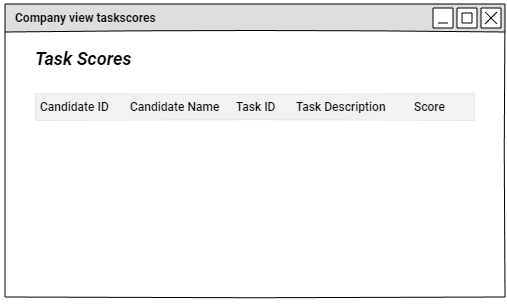
\includegraphics[width=.7\linewidth]{img/company/cmpnytaskviewscr}
	\caption{Task Scores}
\end{figure}

\subsection {Settings}
Change FullName or Password of Company and also Delete Account
\begin{figure}[bph]
	\centering
	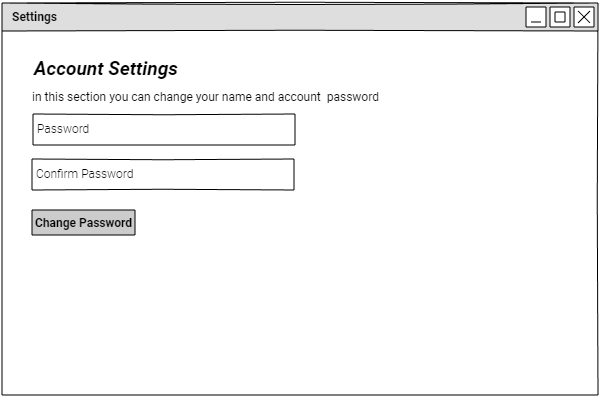
\includegraphics[width=.6\linewidth]{img/company/cmpnystngs}
	\caption{Settings}
\end{figure}
\pagebreak
\addcontentsline{toc}{section}{ - Admin}
\subsection {Admin Homepage}
Overview of Job Portal with Registered Companies, User, Job Post, etc.. 
\begin{figure}[bph]
	\centering
	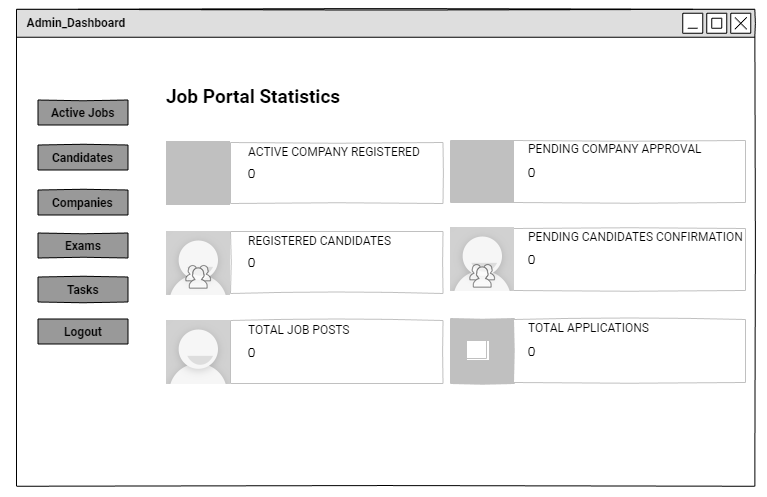
\includegraphics[width=1\linewidth]{img/admin/admindash}
	\caption{Admin Homepage}
\end{figure}


\pagebreak

\subsection {Active Jobs}
Show active Jobs from Companies and manage them
\begin{figure}[bph]
	\centering
	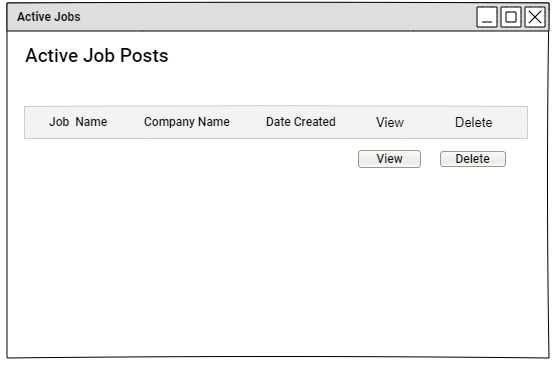
\includegraphics[width=.6\linewidth]{img/admin/adminavtvejobs}
	\caption{Active Jobs}
\end{figure}

\subsection {Candidates}
Show candidates details
\begin{figure}[bph]
	\centering
	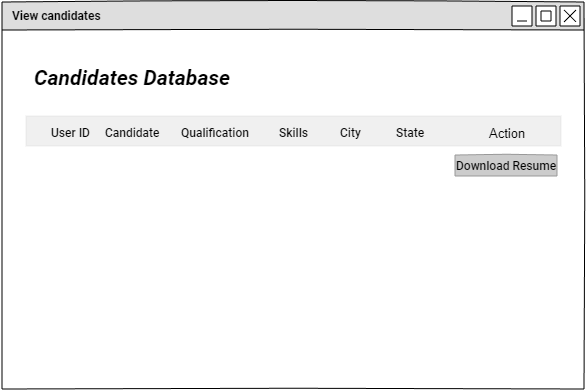
\includegraphics[width=.6\linewidth]{img/admin/adminviewcandidts}
	\caption{Candidates}
\end{figure}
\pagebreak

\subsection {Companies}
Show company details and manage them
\begin{figure}[bph]
	\centering
	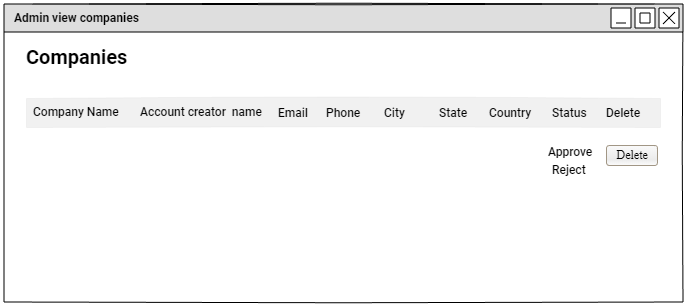
\includegraphics[width=.8\linewidth]{img/admin/adminviewcmpny}
	\caption{Companies}
\end{figure}

\subsection {Exams}
Show details of exams
\begin{figure}[bph]
	\centering
	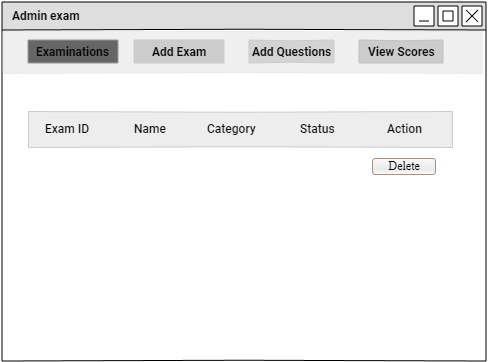
\includegraphics[width=.6\linewidth]{img/admin/adminexam}
	\caption{Exams}
\end{figure}
\pagebreak

\subsection {Add Exams}
Add exams for users
\begin{figure}[bph]
	\centering
	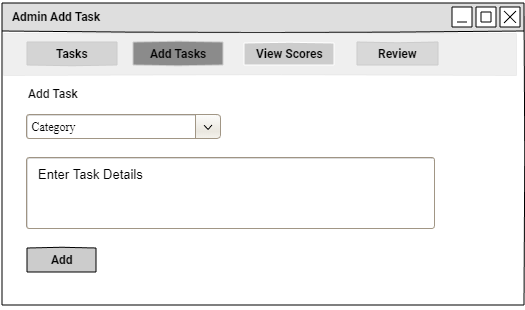
\includegraphics[width=.5\linewidth]{img/admin/adminaddtasks}
	\caption{Add Exams}
\end{figure}

\subsection {Add Questions}
Add Questions for Exams
\begin{figure}[bph]
	\centering
	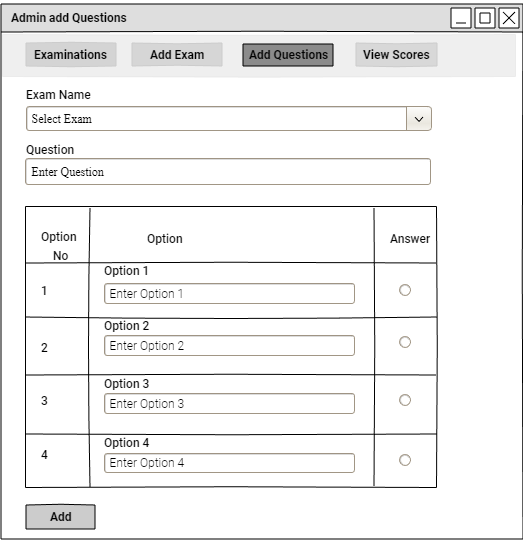
\includegraphics[width=.5\linewidth]{img/admin/adminaddqstns}
	\caption{Add Questions}
\end{figure}
\pagebreak


\subsection {View Scores}
View Scores of Exams
\begin{figure}[bph]
	\centering
	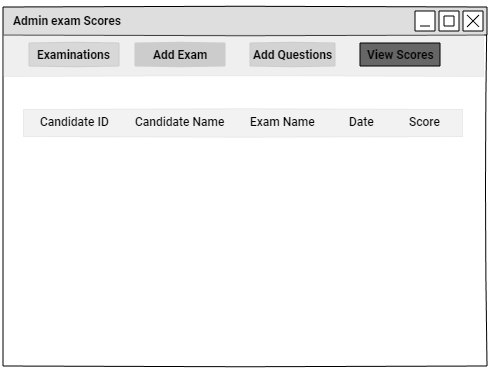
\includegraphics[width=.55\linewidth]{img/admin/adminviewscores}
	\caption{View Scores}
\end{figure}

\subsection {Tasks}
Show Tasks for users
\begin{figure}[bph]
	\centering
	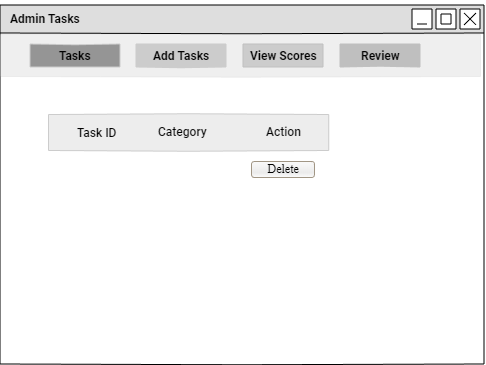
\includegraphics[width=.55\linewidth]{img/admin/admintasks}
	\caption{Tasks}
\end{figure}
\pagebreak

\subsection {Add Tasks}
Add New Tasks
\begin{figure}[bph]
	\centering
	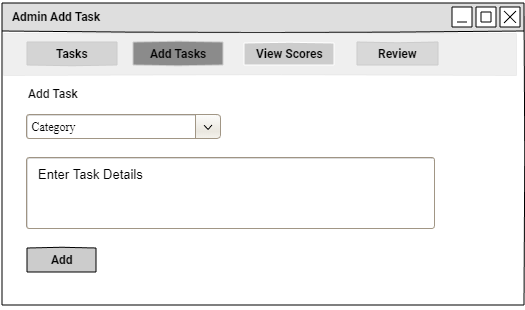
\includegraphics[width=.6\linewidth]{img/admin/adminaddtasks}
	\caption{Add Tasks}
\end{figure}

\subsection {View Scores}
View Task Scores for Users
\begin{figure}[bph]
	\centering
	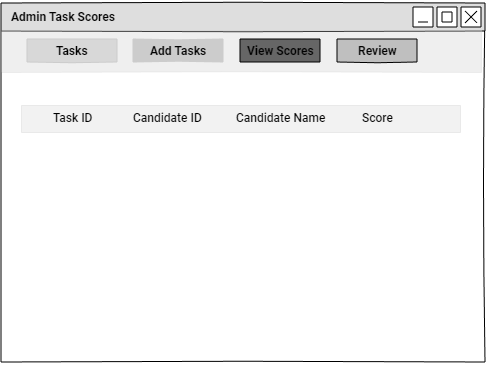
\includegraphics[width=.6\linewidth]{img/admin/admintaskviewscores}
	\caption{View Scores}
\end{figure}
\pagebreak

\subsection {Task Review}
Review tasks done by users
\begin{figure}[bph]
	\centering
	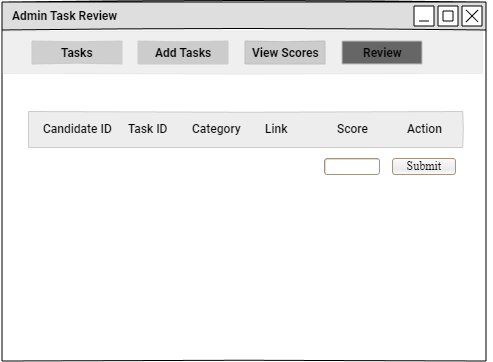
\includegraphics[width=.8\linewidth]{img/admin/admintaskreview}
	\caption{Task Review}
\end{figure}

\pagebreak

\end{document}
